%	LaTeX template for the Collaborative Research Center proposal (3rd funding period) Oxyflame.
%	WSA, RWTH Aachen, 2020, (contact person: Stefan Pielsticker)

%%%% PLEASE ADJUST:
%\WorkInstruction{ Enter the number of the project here. Replace only the text "Example project" Please make sure that the project name corresponds exactly to the name of the folder of your project.}
% Example: \renewcommand{\Project}{A1}

\renewcommand{\Project}{A1}
\renewcommand{\ChapterTitle}{Gas-phase kinetic modelling}
\renewcommand{\ProjectTitle}{Original title from DFG proposal}

%\newcommand*\positioncircle[1]{\raisebox{.5pt}{\textcircled{\raisebox{-.9pt} {#1}}}}


%%%% DON'T CHANGE ANYTHING FROM HERE UNTIL NEXT MARKER!
\chapter{\ChapterTitle}
\label{chap:gas-modelling}
%%%% DONT CHANGE ANYTHING UNTIL HERE!

%%%% PLEASE ADJUST:
\chapterauthor[1]{Anita Meraviglia}
\chapterauthor[1]{Pooria Farmand}
\chapterauthor[1]{Bingjie Chen}
\chapterauthor[2]{Leon Loni Berkel}
\chapterauthor[3]{Stefan Pielsticker}
\chapterauthor[3]{Reinhold Kneer}
\chapterauthor[2]{Christian Hasse}
\chapterauthor[1]{Heinz Pitsch}

%%%% DON'T CHANGE ANYTHING FROM HERE UNTIL NEXT MARKER!
\begin{affils}
	%%%% DONT CHANGE ANYTHING UNTIL HERE!
	
	%%%% PLEASE ADJUST:
	\chapteraffil[1]{\RWTHITV}
	\chapteraffil[2]{\TUDSTFS}
	\chapteraffil[3]{\RWTHWSA}
	
%%%% DON'T CHANGE ANYTHING FROM HERE UNTIL NEXT MARKER!
\end{affils}
\begin{refsection}

\begin{abstract}
\label{sec:\Project _Abstract}
%%%% DONT CHANGE ANYTHING UNTIL HERE!

%%%% PLEASE ADJUST
%\WorkInstruction{Title: Keep it short and make sure that it fits well with the part title and the other project titles within that part. Therefore see the planned chapter outline in section~\ref{ex: chap Outline}.}

%\WorkInstruction{Author List: If you use data from FP1/FP2 members, please list them here as well.}

%\WorkInstruction{Affiliations: Please use the commands already prepared (\textbackslash RWTHWSA, \textbackslash RWTHAIA, \textbackslash RWTHITV, \textbackslash RUBLEAT, \textbackslash RUBLTC, \textbackslash RUBThermo, \textbackslash RUBTC, \textbackslash RUBACII, \textbackslash TUDSTFS,\textbackslash TUDRSM, \textbackslash TUDEST. For changes or other affiliations text us.}

% Abstract
This chapter provides skeletal chemical kinetic models for the gas phase that can be coupled with a detailed solid particle model to describe solid fuel combustion under oxy-fuel conditions. Extensively validated detailed chemical kinetic models are applied and reduced in a multi-step reduction approach to develop skeletal kinetic models for coal and biomass combustion gas-phase kinetics. The obtained chemical kinetic models are validated according to their reduction goal for application in simulations under fuel-lean, high-temperature, and atmospheric pressure conditions. To analyse \ce{NO_x} formation, a \ce{NO_x} sub-model is developed and coupled with a detailed solid particle model for nitrogen release. Furthermore, the role of secondary gas-phase reactions and their consequences for determining kinetic parameters is tackled. In particular, a comparison between experimental and numerical results has been performed. A fluidised bed reactor was chosen as the experimental setup to be investigated due to high gas residence times under hot conditions, which favor gas-phase reactions.

\end{abstract}



\newpage
\section{Introduction} 
Chemical kinetic models are essential when dealing with combustion phenomena as they provide crucial information regarding reaction rates, species transport, and heat transfer effects. Numerical simulations are performed to analyse the partially premixed flame resulting from the combustion of solid coal and biomass particles. These numerical simulations are conducted predominantly under high-temperature air and oxy-fuel conditions at atmospheric pressure, which are relevant to practical applications. Therefore, with this application in mind, it is necessary to develop a chemical kinetic model to describe the underlying chemistry of the released volatile species in the surrounding gas phase of the solid particle. The volatile species are determined by employing the solid particle model for coal and biomass devolatilisation from chapter 8, which leads to the definition of a complex mixture ranging from light hydrocarbons and oxygenated species up to heavy lignin tars (\ce{C24H28O4}) and aromatic compounds. 
Concerning the \ce{NO_x} sub-model from chapter 8, several nitrogen-containing species are released into the gas phase. The inclusion of the appropriate chemical reactions describing their behaviour in the combustion system is essential to capture the primary \ce{NO_x} formation pathways in the kinetic model.
\\
Detailed chemical kinetic models aim to describe the combustion process as accurately as possible. However, this might require hundreds or even thousands of species and reactions. The computational cost of simulations typically increases with the number of species in the employed kinetic models. Therefore, developing skeletal kinetic models with a reduced number of species and reactions, while preserving high accuracy, is of key importance for performing the simulations that would be otherwise computationally prohibitive.
\\
According to the literature, present kinetic models for coal and biomass combustion are either not adapted to the solid particle model from chapter 8, do not contain large aromatic species, or are not validated for the application under oxy-fuel conditions~\cite{Shamooni2021, Goyal2017, Lovas2013}. In addition, most of the kinetic models for \ce{NO_x} formation do not contain all the volatile species released from the solid nitrogen particle model like the model from Glarborg et al.~\cite{Glarborg2018} or are not well documented~\cite{Shamooni2021}. 
\\
Another important aspect related to gas-phase kinetics is the impact that the gas residence of the volatile products formed during the primary pyrolisis has on the decomposition of the secondary pyrolysis products due to gas-phase reactions. On the experimental side, the fluidised bed reactor is an excellent candidate to investigate this phenomenon, due to its high residence times under hot conditions. A numerical analysis has also been performed. The models chosen for the comparison are the CRECK-G-2003 and the Bio-CPD. In the CRECK-G-2003, two different sets of parameters for the first-order tar cracking model have been used (\cite{Fagbemi2001, Pielsticker2024}).

%The development of chemical kinetic models for the gas phase kinetics coupled with the solid particle model from Chapter~\textbf{Solid Fuel Conversion} is presented in this chapter. 
The present chapter is structured as follows. The first part delves into the development process of skeletal coal and biomass combustion models and of a modular \ce{NO_x} model, while the second part focuses on the validation of the aforementioned models. The last part aims to describe the importance of secondary gas-phase reactions in experimental setups.


\newpage
\section{Chemical kinetic model development}
The development of chemical kinetic models for coal and biomass combustion is presented in this section. A reduced version of the model from Cai et al.~\cite{Cai2020} is developed for coal combustion. According to this model, the development of recent kinetic models for coal and biomass combustion is discussed. These recently developed models are built to be adapted to the solid particle model from chapter 8. Furthermore, a modular \ce{NO_x} model is developed based on the solid particle model and is presented at the end of this section.


\subsection{Development of skeletal coal and biomass models}

A skeletal kinetic model for coal combustion was developed by Cai et al.~\cite{Cai2019}. Based on the detailed kinetic model from Blanquart et al.~\cite{Blanquart2009}, it describes the oxidation of a set of \ce{C0} to \ce{C4} hydrocarbon fuels including \ce{CH4}. This base-chemistry is extended to include the formation of polycyclic aromatic hydrocarbon according to the study from Narayanaswamy et al.~\cite{Narayanaswamy2010} and is refined by incorporating the hydrogen mechanism from Burke et al.~\cite{Burke2012}. Further details about the development process can be found in~\cite{Cai2019,Cai2020}. The model from Cai et al.~\cite{Cai2020} is extensively validated for the combustion of fuels in air~\cite{Cai2019} and for the oxy-methane combustion~\cite{Cai2020}. In this chapter, this kinetic model will be named ITV-2019, and it is developed and validated for the ignition delay time, the laminar burning velocity, and the extinction strain rate of \ce{CH4} under air and oxy-fuel conditions. A description of the extinction strain rate measurements is given in Chapter~\ref{chap:gas-phase-exp}.
\\
An update of the ITV-2019 model with a revised base chemistry has been developed by Langer et al.~\cite{Langer2023} (ITV2023-Base-Chemistry). From this, recently developed skeletal kinetic models for coal (Skeletal-ITV-Coal) and biomass (Skeletal-ITV-Bio) combustion are tailored to the solid particle model from chapter 8. These models are developed to predict the ignition delay time and the respective fuel chemistry to simulate the gas-phase kinetics under high-temperature and atmospheric pressure conditions. Developing these recent skeletal kinetic models for coal and biomass combustion involves a multi-step reduction strategy using detailed chemical kinetic models. A schematic of the whole reduction strategy is summarized in Fig.~\ref{fig:B1bKineticModelDevelopmentStructure}.
% Mechanism development strategy
\begin{figure}[h]
  \centering
  \subfloat{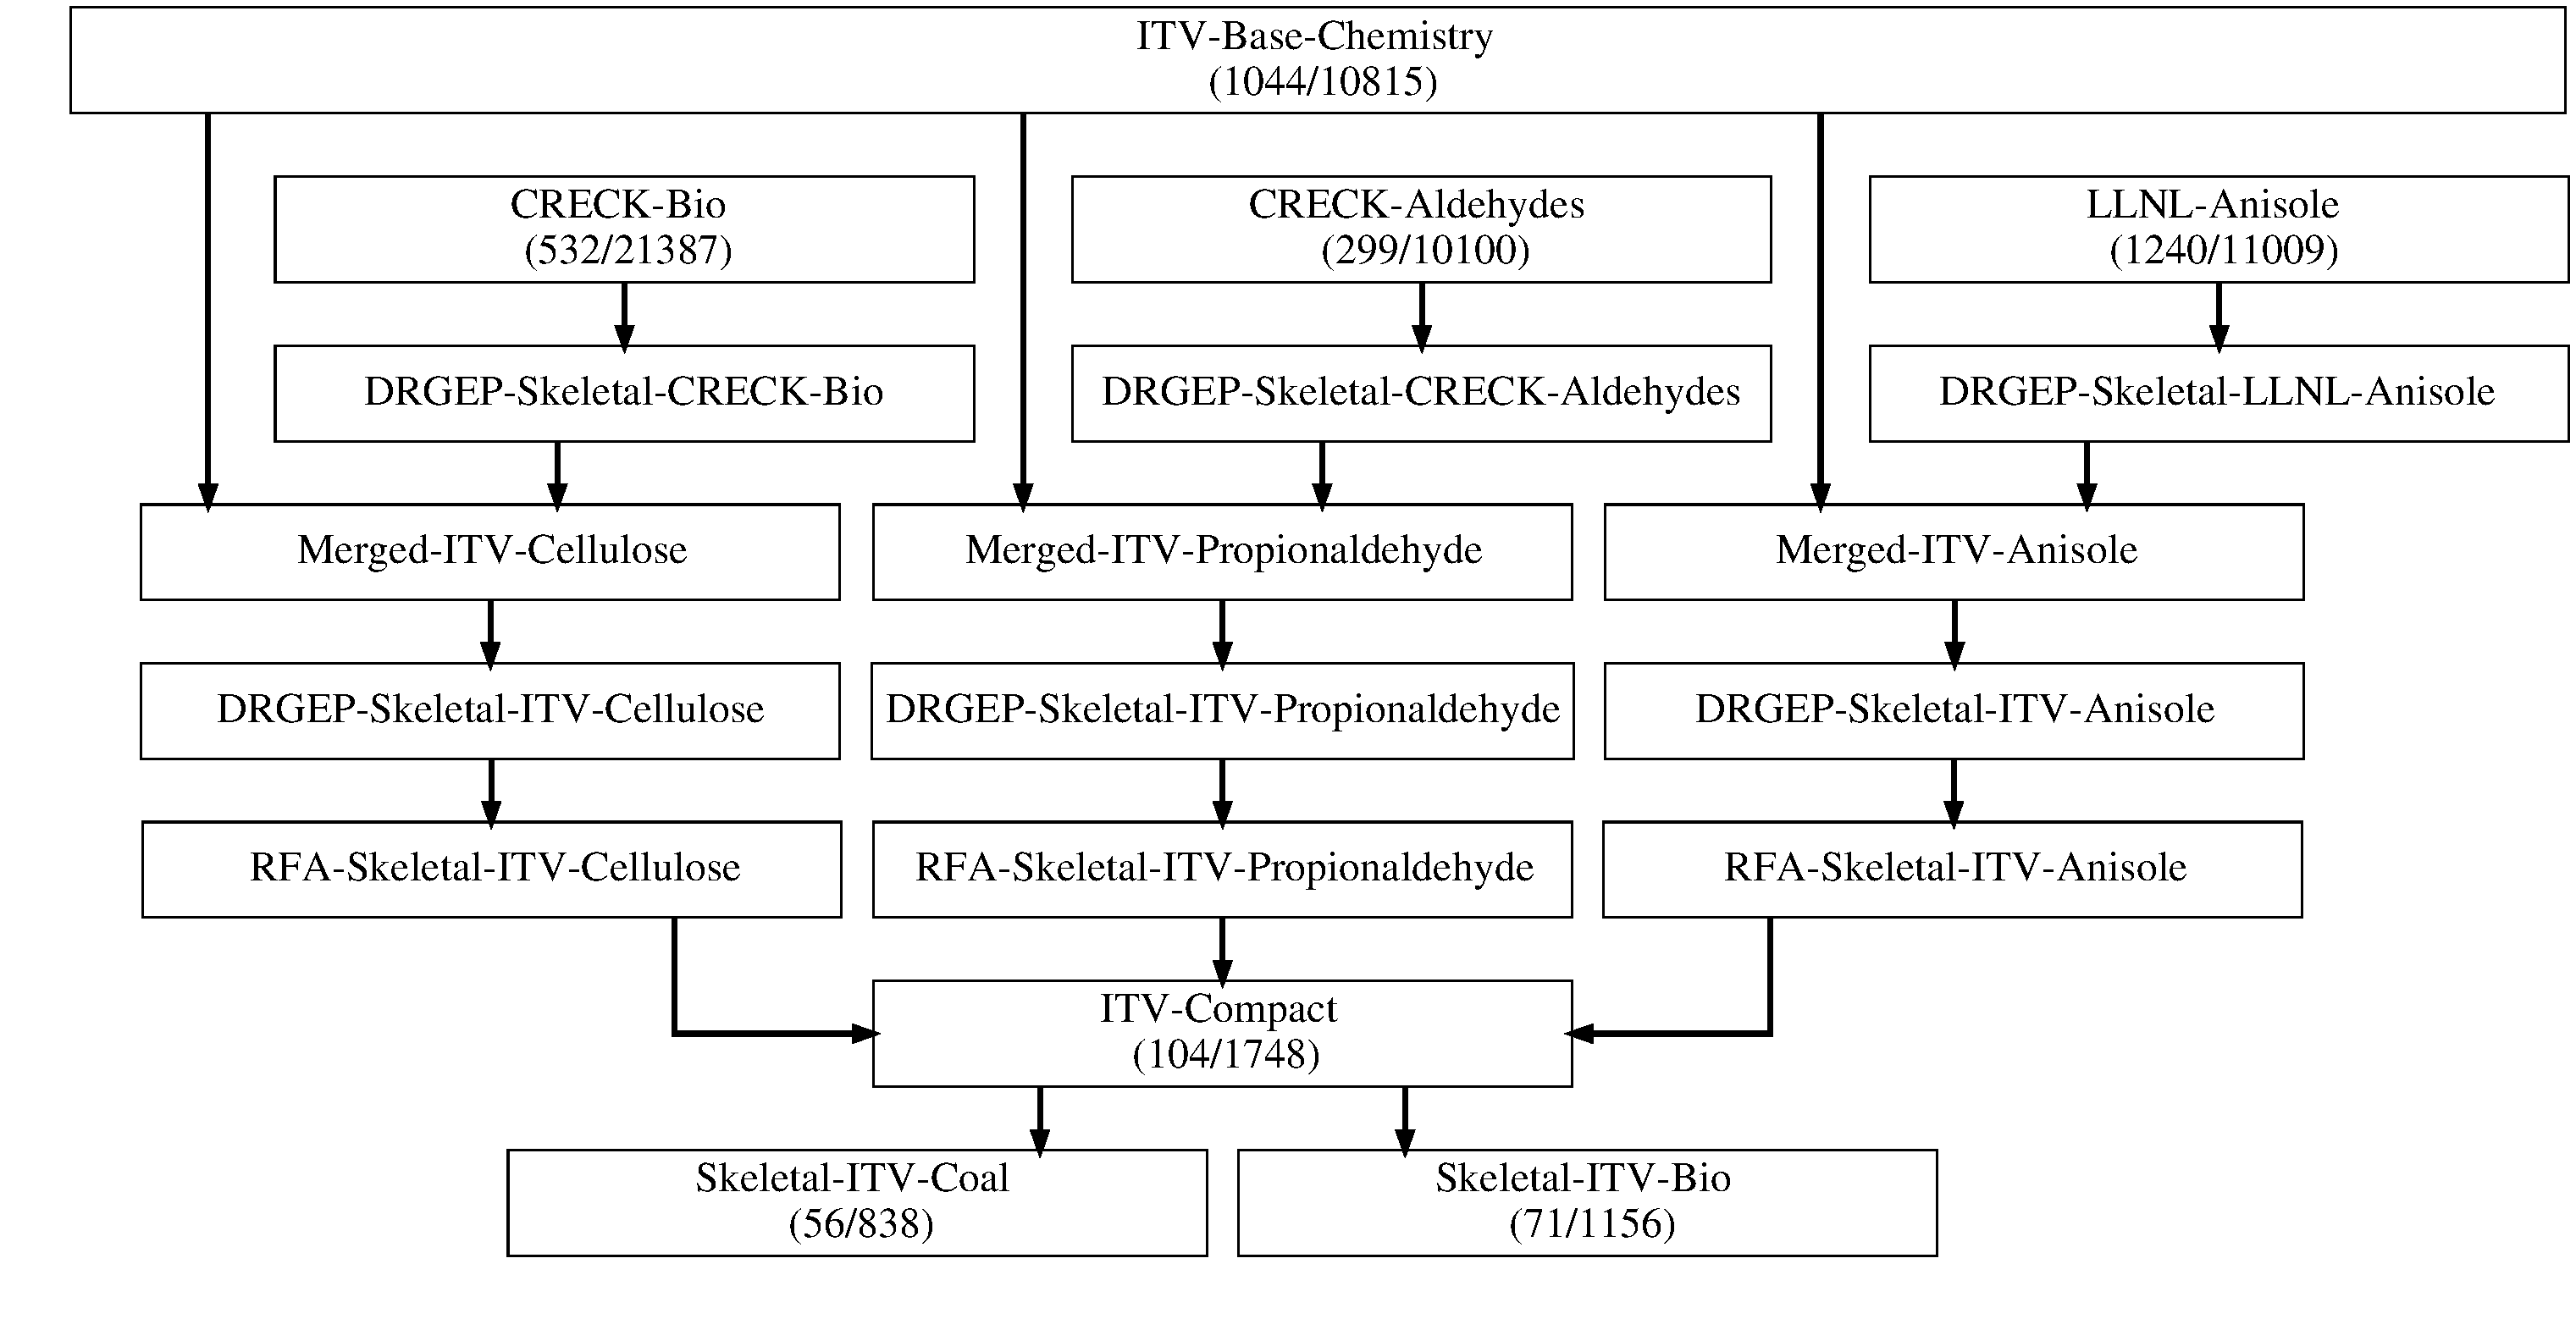
\includegraphics[width=1.0\textwidth]{\ThisPath Figures/B1b_FlowChartMechanismDevelopment.pdf}}
  \caption{Flow chart for developing the skeletal gas phase mechanisms for coal (Skeletal-ITV-Coal) and biomass (Skeletal-ITV-Bio) combustion. The initial mechanisms are the ITV2023-Base-Chemistry from Langer et al.~\cite{Langer2023}, the CRECK-Bio~\cite{Debiagi2016}, the CRECK-Aldehydes~\cite{Pelucchi2015}, and the LLNL-Anisole model~\cite{Wagnon2018}. Number of species and reactions are indicated in parenthesis.}
  \label{fig:B1bKineticModelDevelopmentStructure}
\end{figure}
\\
According to the devolatisation models from chapter 8, coal and biomass particles release a complex mixture of volatile species to the gas-phase. One of the dominant volatile species released during lignin combustion is anisole, while levoglucosan is the dominant volatile species released from cellulose combustion. To describe the ignition delay time of coal and biomass combustion, the chemistry of anisole and levoglucosan - the most dominant species released at particle temperatures where biomass ignites - is considered based on model simulations with the solid particle model from chapter 8. However, these species are not included in the extensively validated ITV2023-Base-Chemistry model~\cite{Langer2023}. To integrate the missing species' chemistry in the ITV2023-Base-Chemistry, extensively validated detailed chemical kinetic models are used to describe the respective chemistry of interest over a broad range of conditions. The missing anisole chemistry has been adopted from the model of Wagnon et al.~\cite{Wagnon2018}, cellulose volatile species from Debiagi et al.~\cite{Debiagi2016}, and the propionaldehyde chemistry from Pelucchi et al.~\cite{Pelucchi2015}.
\\
The integration of the chemistry describing the gas-phase kinetics of these volatile species into the ITV2023-Base-Chemistry has been achieved using a systematic approach. To extrapolate only the relevant chemistry for the species, the Direct Relation Graph with Error Propagation (DRGEP) method~\cite{PepiotDesjardins2008} has been applied to these detailed models. The obtained reduced chemical kinetic models are then merged into ITV2023-Base-Chemistry. Only the species and reactions, as well as the species thermodynamic and transport data, are extracted and added to the model.
\\
The obtained kinetic models are referred to as \textit{Merged-ITV-Cellulose}, \textit{Merged-ITV-Propionaldehyde}, and \textit{Merged-ITV-Anisole}, as shown in Fig.~\ref{fig:B1bKineticModelDevelopmentStructure}. The obtained models undergo a multi-step reduction strategy involving the DRGEP method~\cite{PepiotDesjardins2008a} followed by Reaction Flux Analysis (RFA). A reaction flux analysis allows a flexible and targeted extraction of major formation and consumption pathways of the species of interest from the mechanism, while the DRGEP method~\cite{PepiotDesjardins2008a} is a more conservative reduction method. The extraction with the reaction flux analysis is performed based on the respective validation cases to consider the range of validity and application. The validation database presented in~\cite{Langer2023} is expanded in this work by integrating additional speciation data representative of anisole oxidation~\cite{Chen2022}, cellulose pyrolisis~\cite{Norinaga2013}, and shock tube ignition-delay time measurements of anisole and propionaldehyde~\cite{Pelucchi2015, AkihKumgeh2011}.
\\
Skeletal kinetic models from each reduction step are named employing the prefixes \textit{DRGEP-Skeletal} and \textit{RFA-Skeletal} in Fig.~\ref{fig:B1bKineticModelDevelopmentStructure}, followed by the name of the corresponding detailed chemical kinetic model. The reduction process allows the retention of only the relevant chemistry for the species of interest. This allows the merging process of the skeletal models to be more straightforward, leading to a compact chemical kinetic model (ITV-Compact) which is able to accurately describe the evolution of the volatile species released from coal and biomass.
\\
The final reduction step contains a DRGEP step and an additional reduction step using the reaction flux analysis to obtain skeletal chemical kinetic models for coal and biomass combustion. These skeletal kinetic models describe the gas phase kinetics of volatile species released from coal (Skeletal-ITV-Coal) and biomass (Skeletal-ITV-Bio). The applicability of both models can be emphasized by the fact that the Skeletal-ITV-Coal and the Skeletal-ITV-Bio mechanisms contain several volatile species released from the solid particle model from chapter 8.


\subsection{Development of a \ce{NOx} chemical kinetic sub-model}

To describe the formation of \ce{NO_x} from nitrogen-containing volatile species released from the solid particle model from chapter 8, a new chemical kinetic gas phase model for \ce{NO_x} formation is developed. This chemical kinetic model is based on an ITV-\ce{NO_x} model, a reduced version of the Glarborg model~\cite{Glarborg2018}, crafted through ab initio and experimental studies, as base chemistry. As a result of Girhe et al.~\cite{Girhe2024}, the ammonia chemistry from the KAUST model~\cite{Zhang2023} is integrated into the ITV-\ce{NO_x} model to improve the predictions of the ammonia chemistry. The \ce{C5H5N}-chemistry, which is employed to model tar-N, is adopted from the CRECK-\ce{NO_x} model~\cite{Shamooni2021} and integrated into the base-chemistry model.
\\
A reaction rate modification is applied since this merged ITV-\ce{NO_x} model over-predicts the \ce{NO} formation over a broad range of experimental conditions. A rate parameter adoption from the CRECK-\ce{NO_x} model~\cite{Shamooni2021} (reaction: $\ce{NCO}+\ce{O} \Leftrightarrow \ce{NO}+\ce{CO}$) and a minor tuning of the frequency parameter (reaction: $\ce{NCO}+\ce{NO} \Leftrightarrow \ce{N2O}+\ce{CO}$) result in an accurate prediction of the \ce{NO} chemistry (Complete-ITV2023-\ce{NO_x}).
\\
After the rate modifications, the nitrogen chemistry in the Complete-ITV2023-\ce{NO_x} model is extracted using the reaction flux analysis to obtain a more compact model size. Considering the validation cases from Alzueta et al.~\cite{Alzueta2002} and Wu et al.~\cite{Wu2019, Wu2022}, a modular Skeletal-ITV-\ce{NO_x} kinetic model is obtained, which covers a broad spectrum of fuel-air ratios, temperatures, and initial conditions with 36 species and 595 reactions.

\newpage
\section{Validation of kinetic models}

The skeletal chemical kinetic models are developed to predict the ignition delay time and the respective fuel chemistry based on detailed chemical kinetic models. However, due to the reduction of detailed chemical kinetic models, the prediction accuracy of the chemistry of several species is affected. Consequently, a comprehensive validation is required to cover all relevant fuels and target species, including ignition delay times and speciation data across a broad range of temperatures at atmospheric pressure. Numerical simulations for validation are performed using appropriate models in the FlameMaster code~\cite{Pitsch1998b}.


\subsection{Skeletal kinetic models for coal combustion}

This subsection provides a validation of the ITV-2019 kinetic model for coal combustion and the ITV-2023 models for coal and biomass combustion, covering all aspects of the respective development goals.
\\
The ITV-2019 coal model is developed for an accurate prediction of the oxy-methane chemistry. Figure~\ref{fig:B1bIDTLimingCaiCoalMechanism} shows model predictions of the ITV-2019 model in comparison with experimental shock-tube measurements from Koroglu et al.~\cite{Koroglu2016}. Koroglu et al.~\cite{Koroglu2016} measured the ignition delay time for \ce{CH4}/\ce{O2}/\ce{CO2} mixtures in bath gas of \ce{Ar} for different pressures and equivalence ratios. As shown in Fig.~\ref{fig:B1bIDTLimingCaiCoalMechanism}, the ITV-2019 model satisfactorily predicts the ignition delay times for all conditions and temperature ranges.
% Ignition delay time validation - Koroglu
\begin{figure}[h]
  \centering
  \subfloat{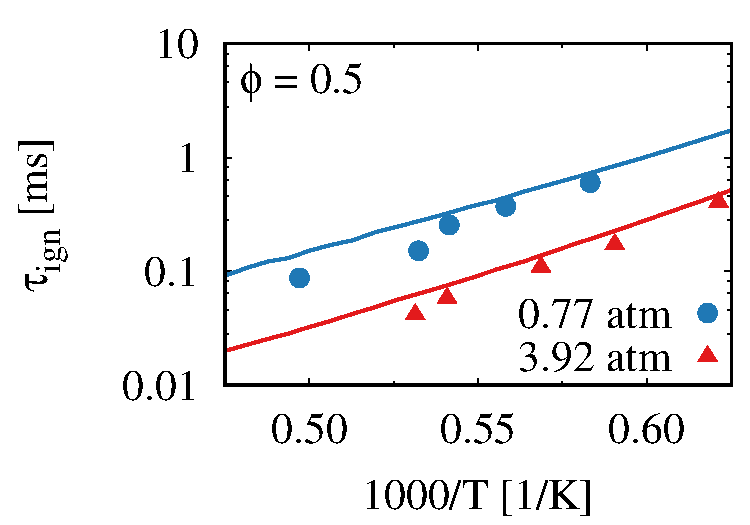
\includegraphics[width=0.32\textwidth]{\ThisPath Figures/B1b_LCai_IDT_CH4_Koroglu_Lean.pdf}}
  \hfill
  \subfloat{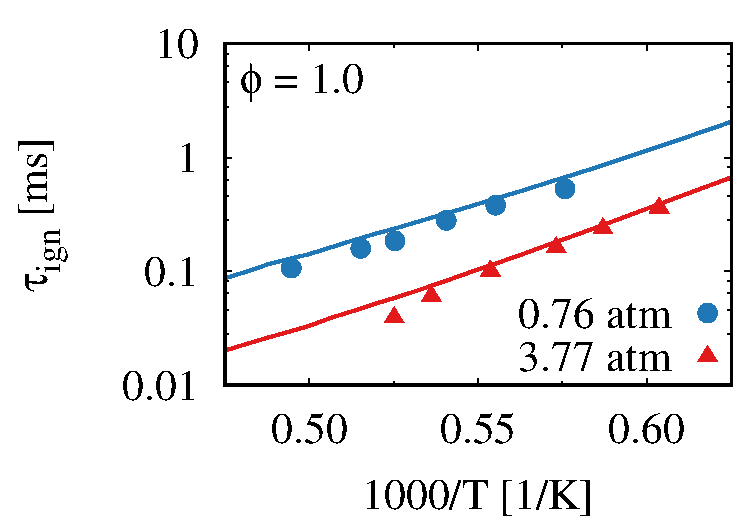
\includegraphics[width=0.32\textwidth]{\ThisPath Figures/B1b_LCai_IDT_CH4_Koroglu_Stoi.pdf}}
  \hfill
  \subfloat{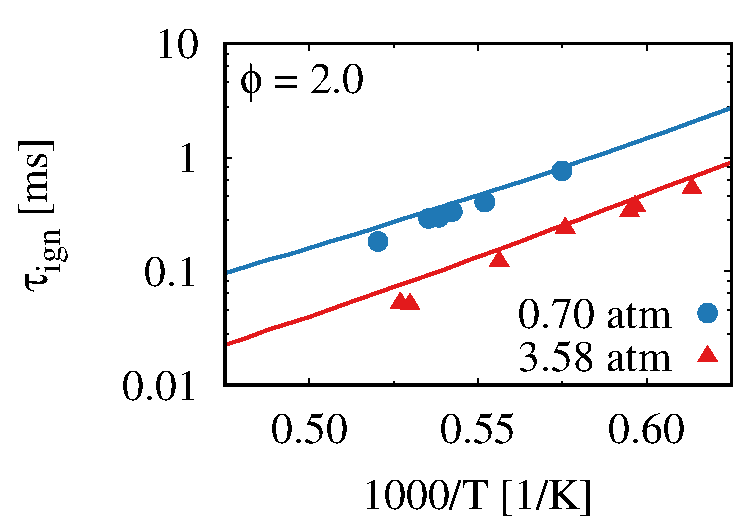
\includegraphics[width=0.32\textwidth]{\ThisPath Figures/B1b_LCai_IDT_CH4_Koroglu_Rich.pdf}}
  \caption{Comparison of experimentally measured ignition delay times of \ce{CH4}/\ce{O2}/\ce{CO2}/\ce{Ar} mixtures from Koroglu et al.~\cite{Koroglu2016} (symbols) with model predictions of the ITV-2019 model (lines) for different equivalence ratios.}
  \label{fig:B1bIDTLimingCaiCoalMechanism}
\end{figure}
% Ignition delay time validation - Maruta
\begin{figure}[t]
  \centering
  \subfloat{\includegraphics[width=0.32\textwidth]{\ThisPath Figures/B1b_LCai_ExtStr_a.pdf}}
  \hfill
  \subfloat{\includegraphics[width=0.32\textwidth]{\ThisPath Figures/B1b_LCai_ExtStr_b.pdf}}
  \hfill
  \subfloat{\includegraphics[width=0.32\textwidth]{\ThisPath Figures/B1b_LCai_ExtStr_c.pdf}}
  \caption{Comparison of experimentally measured extinction strain rates (symbols) and model predictions of the ITV-2019 model (lines). Each plot refers to a different oxygen mole fractions.}
  \label{fig:B1bExtStrainRateLimingCaiCoalMechanism}
\end{figure}
\\
In addition to the ignition delay time validation, the ITV-2019 model is also validated for the extinction strain rate. Figure~\ref{fig:B1bExtStrainRateLimingCaiCoalMechanism} compares the model prediction of the kinetic model with experimentally measured extinction strain rates of diffusion flames with \ce{CH4}/\ce{CO2} (\SI{300}{K}) and \ce{O2}/\ce{CO2} (\SI{310}{K}) streams. The ITV-2019 model predicts the extinction strain rate in good agreement with the experimental data. Details about the extinction strain rate experiment can be found in chapter~\ref{chap:gas-phase-exp}. Further validation cases, including the laminar burning velocity, are presented in~\cite{Cai2020}.
% Ignition delay time validation
\begin{figure}[b]
  \centering
  \subfloat{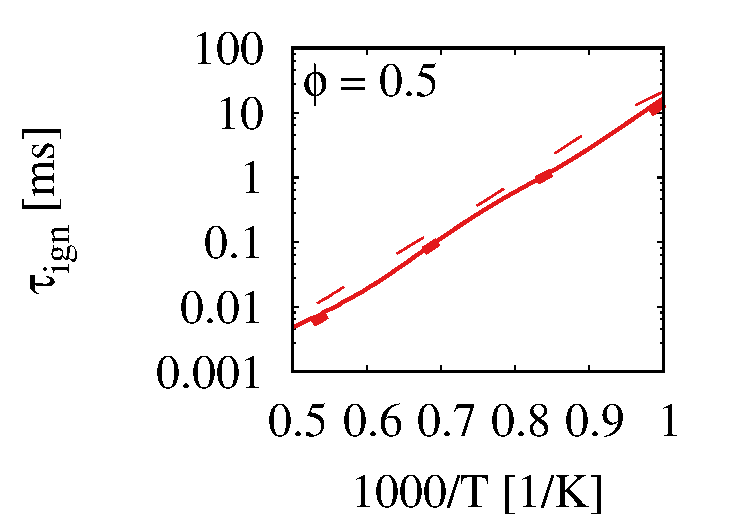
\includegraphics[width=0.32\textwidth]{\ThisPath Figures/B1b_Coal_IDT_Lean_1atm.pdf}}
  \hfill
  \subfloat{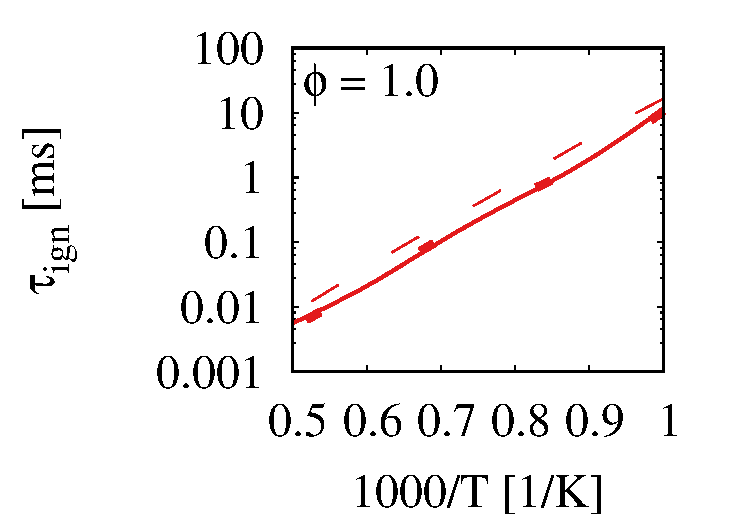
\includegraphics[width=0.32\textwidth]{\ThisPath Figures/B1b_Coal_IDT_Stoichiometric_1atm.pdf}}
  \hfill
  \subfloat{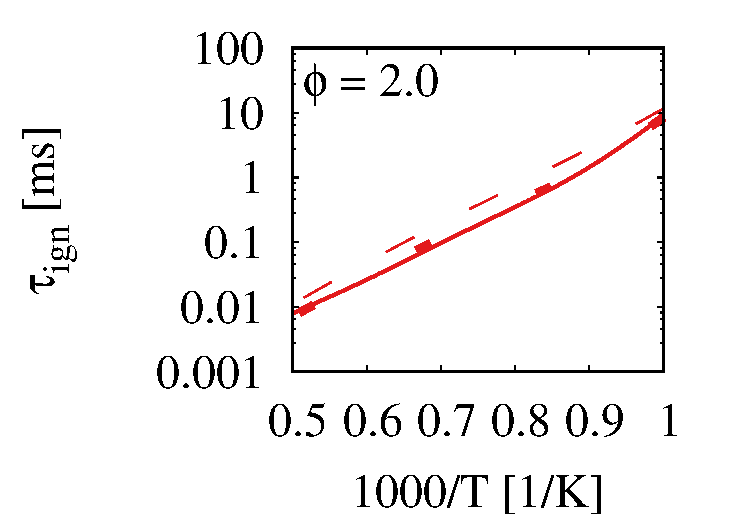
\includegraphics[width=0.32\textwidth]{\ThisPath Figures/B1b_Coal_IDT_Rich_1atm.pdf}}
  \caption{Model comparison for the ignition delay times of anisole/air mixtures at atmospheric pressure for the Skeletal-ITV-Coal model (solid lines), the Merged-ITV-Anisole model (dotted lines), and the LLNL-Anisole model~\cite{Wagnon2018} (dashed lines) for different equivalence ratios.}
  \label{fig:B1bIDTAnisoleCoalMechanism}
\end{figure}
\\
The ITV-2023 coal skeletal model is validated by considering the oxidation of anisole at atmospheric pressure over a broad range of temperatures. Quantities predicted by the skeletal model are compared against the ones of the corresponding detailed model to assess the effect induced by the reduction phase. Additionally, to assess the influence of differing base chemistries, the performance of the ITV-based detailed chemical kinetic model is evaluated against both the reference models and, where possible, experimental data. The detailed chemical kinetic model from Wagnon et al.~\cite{Wagnon2018} and the Merged-ITV-Anisole mechanism serve as a reference for the skeletal chemical kinetic model in both cases.
% Ansiole oxidation chemistry - oxy conditions
\begin{figure}[t]
  \centering
  \subfloat{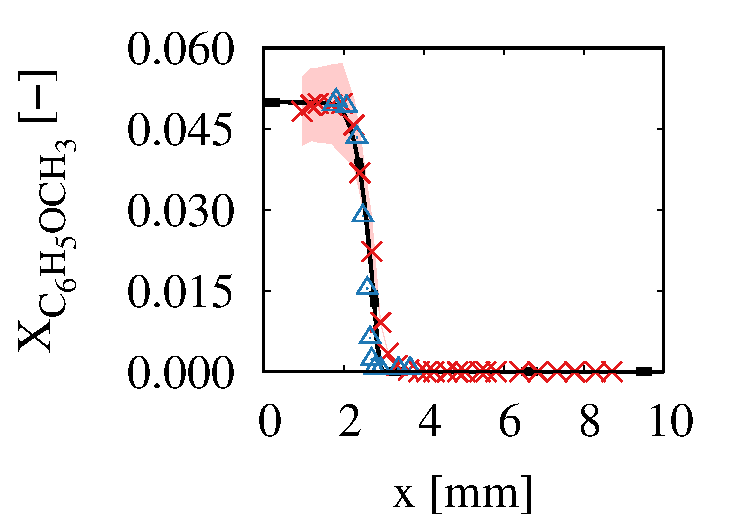
\includegraphics[width=0.32\textwidth]{\ThisPath Figures/B1b_Coal_Figure_6a.pdf}}
  \hfill
  \subfloat{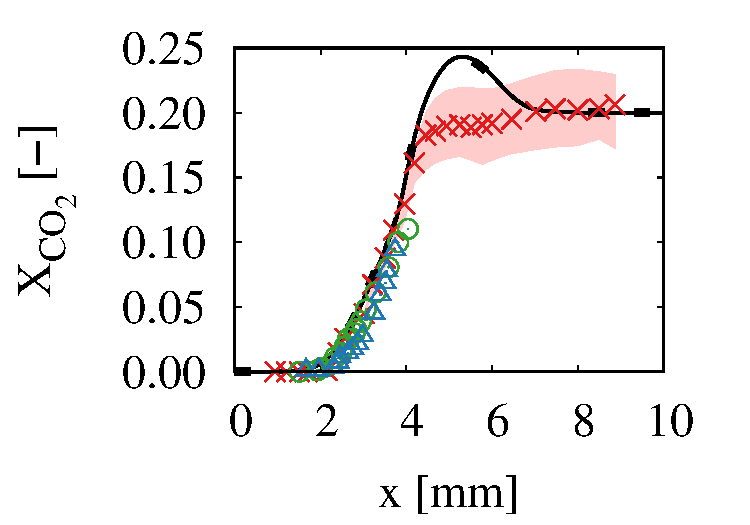
\includegraphics[width=0.32\textwidth]{\ThisPath Figures/B1b_Coal_Figure_6f.pdf}}
  \hfill
  \subfloat{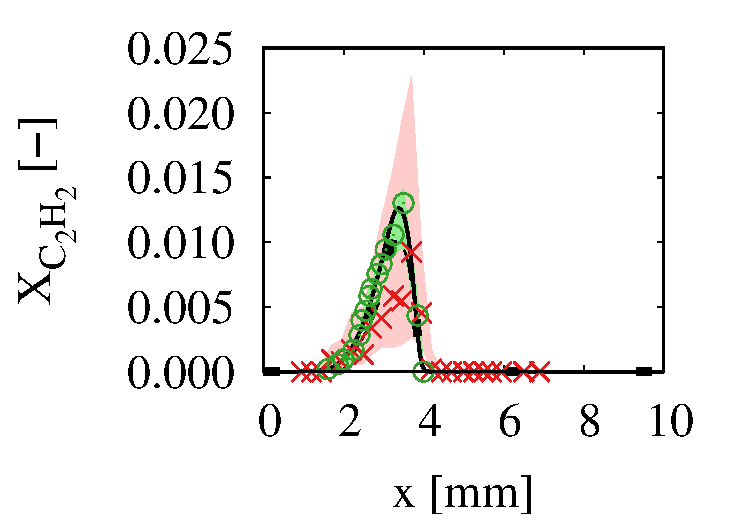
\includegraphics[width=0.32\textwidth]{\ThisPath Figures/B1b_Coal_Figure_8b.pdf}}
  \caption{Comparison of experimentally measured mole fractions in the \ce{CO2}-\ce{O2}-Flame for anisole oxidation from Chen et al.~\cite{Chen2022} (Time-of-Flight Molecular Beam Mass Spectrometer (ToF-MBMS): red crosses; Gas Chromatoraph Mass Spectrometer (GC-MS) with a Rt-Q-Bond column: green circles; GC-MS with a DB-Petro column: blue triangles) with model predictions of the Skeletal-ITV-Coal (solid lines), the Merged-ITV-Anisole (dotted lines), and the LLNL-Anisole model~\cite{Wagnon2018} (dashed lines). Shaded areas with different colours indicate the measurement uncertainty of the respective techniques. x refers to the distance from the fuel inlet at 0 mm to the oxidiser inlet at 10 mm.}
  \label{fig:B1bAnisoleOxidationCoalMechanismCO2O}
\end{figure}
\\
Figure~\ref{fig:B1bIDTAnisoleCoalMechanism} compares the model prediction for the ignition delay time of anisole/air mixtures for the Skeletal-ITV-Coal, the Merged-ITV-Anisole, and the LLNL-Anisole~\cite{Wagnon2018} models. Model predictions for the ignition delay times of the Skeletal-ITV-Coal and the Merged-ITV-Anisole model are similar, indicating a low error in the mechanism reduction process. The difference in the prediction of the ignition delay time compared to the LLNL-Anisole model~\cite{Wagnon2018} is based on the different base chemistries in the models.
The validation of the anisole oxidation chemistry for the Skeletal-ITV-Coal model is given based on the experimental study from Chen et al.~\cite{Chen2022}. An examined flame configuration contains carbon dioxide as a diluent on the oxidizer side (\ce{CO2}-\ce{O2}-Flame) to represent oxy-fuel conditions as discussed in chapter~\ref{chap:gas-phase-exp} Figure~\ref{fig:B1bAnisoleOxidationCoalMechanismCO2O} compares the Skeletal-ITV-Coal model predictions with the respective detailed kinetic model predictions in the \ce{CO2}-\ce{O2}-Flame. Anisole and \ce{CO2} model predictions of the Skeletal-ITV-Coal model show no discrepancies to the detailed LLNL-Anisole~\cite{Wagnon2018} and the Merged-ITV-Anisole. Skeletal-ITV-Coal model captures the intermediate \ce{C2H2} species mole fraction peak, measured by the GC-MS. On the other hand, Merged-ITV-Coal and LLNL-Anisole~\cite{Wagnon2018} models both underpredict the \ce{C2H2} peak.


\subsection{Skeletal kinetic model for biomass combustion}

Applying the newly developed skeletal kinetic model for biomass combustion requires a detailed validation of the ignition delay time and the levoglucosan and anisole chemistry in a predefined range of validity. The Skeletal-ITV-Bio model is built on the detailed chemical kinetic models of CRECK-Aldehydes~\cite{Pelucchi2015}, CRECK-Bio~\cite{Debiagi2016}, LLNL-Anisole~\cite{Wagnon2018}, and the updated ITV2023-Base-Chemistry~\cite{Langer2023}. These detailed chemical kinetic models are validated against data from several experimental species over various conditions. The newly developed Skeletal-ITV-Bio kinetic model will be validated for the ignition delay time of propionaldehyde, secondary pyrolysis of cellulose volatile species, and for the anisole oxidation chemistry against experimental data~\cite{Pelucchi2015, AkihKumgeh2011, Chen2022}.
% Ignition delay time validation
\begin{figure}[h]
  \centering
  \subfloat{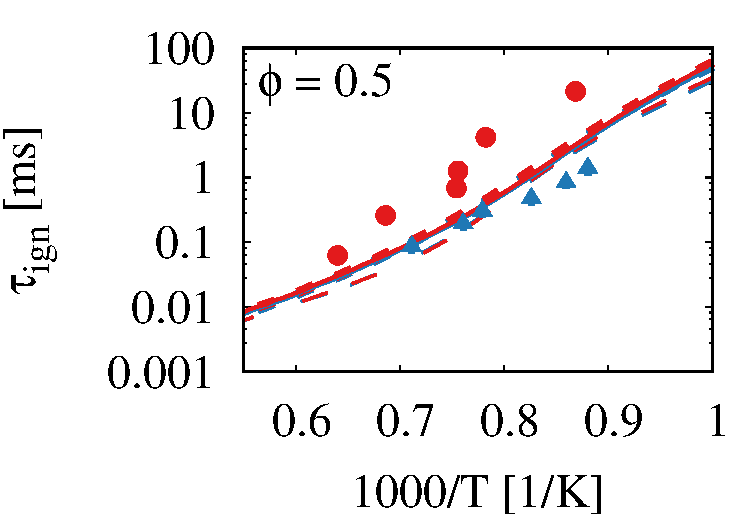
\includegraphics[width=0.32\textwidth]{\ThisPath Figures/B1b_Bio_IDT_Propanal_Lean.pdf}}
  \hfill
  \subfloat{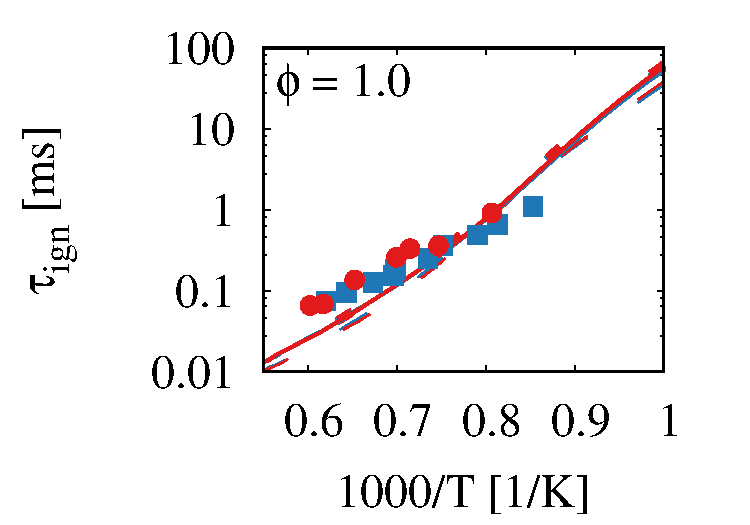
\includegraphics[width=0.32\textwidth]{\ThisPath Figures/B1b_Bio_IDT_Propanal_Stoichiometric.pdf}}
  \hfill
  \subfloat{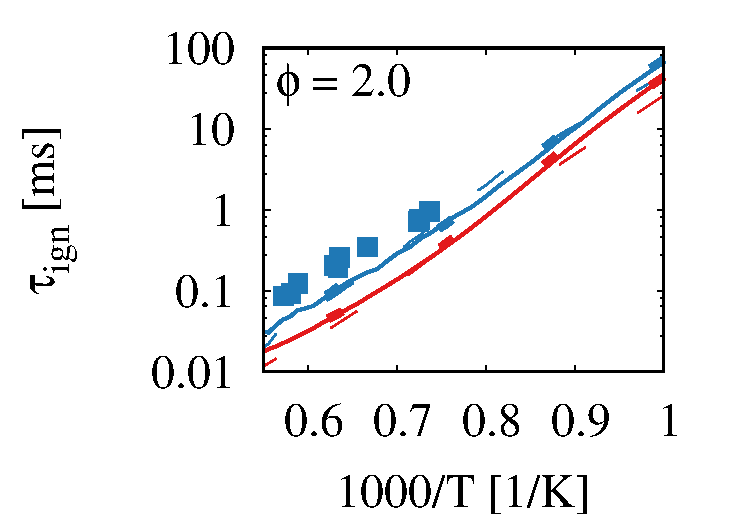
\includegraphics[width=0.32\textwidth]{\ThisPath Figures/B1b_Bio_IDT_Propanal_Rich.pdf}}
  \caption{Comparison of the propionaldehyde ignition delay time for experimental shock-tube measurements from Pelucchi et al.~\cite{Pelucchi2015} (blue squares) and from Akih-Kumgeh and Bergthorson~\cite{AkihKumgeh2011} (red circles) with model predictions of the Skeletal-ITV-Bio model (solid lines), the Merged-ITV-Propionaldehyde model (dotted lines), and the CRECK-Aldehydes model~\cite{Pelucchi2015} (dashed lines) for different equivalence ratios.}
  \label{fig:B1bIDTPropionaldehydeBioMechanism}
\end{figure}
% Cellulose pyrolysis validation
\begin{figure}[b]
  \centering
  \subfloat{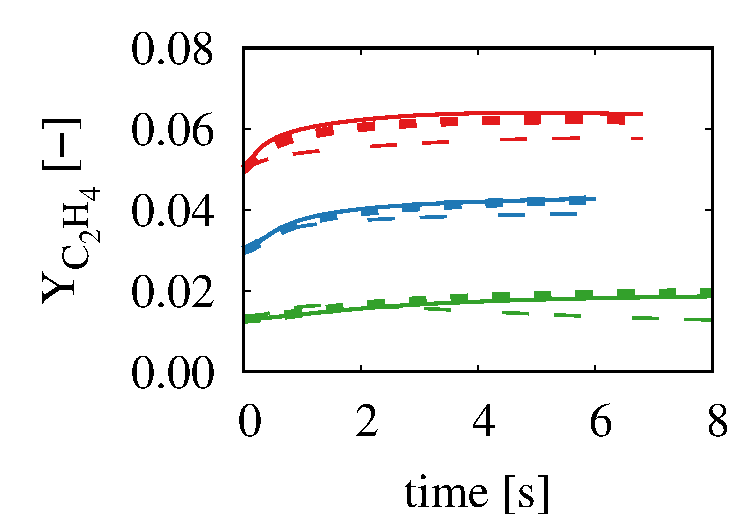
\includegraphics[width=0.32\textwidth]{\ThisPath Figures/B1b_Bio_CellulosePyrolysis_C2H4.pdf}}
  \hfill
  \subfloat{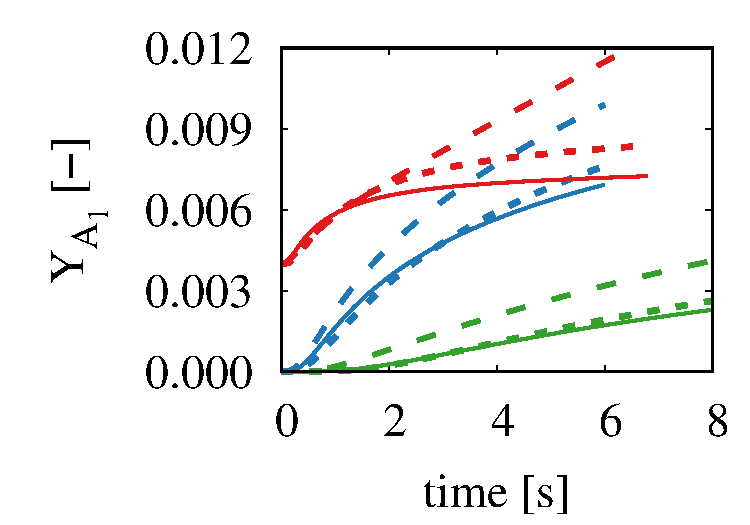
\includegraphics[width=0.32\textwidth]{\ThisPath Figures/B1b_Bio_CellulosePyrolysis_C6H6.pdf}}
  \hfill
  \subfloat{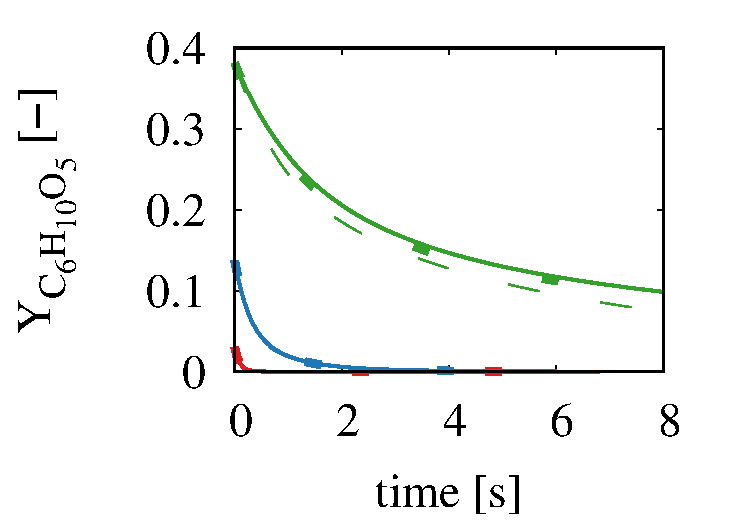
\includegraphics[width=0.32\textwidth]{\ThisPath Figures/B1b_Bio_CellulosePyrolysis_C6H10O5.pdf}}
  \caption{Model comparison for the secondary pyrolysis of cellulose volatile species at \SI{700}{\celsius} (green), \SI{750}{\celsius} (blue), and \SI{800}{\celsius} (red) for the Skeletal-ITV-Bio (solid lines), the Merged-ITV-Cellulose (dotted lines), and the CRECK-Bio model~\cite{Debiagi2016} (dashed lines).}
  \label{fig:B1bCellulosePyrolysisBioMechanism}
\end{figure}
\\
The ignition delay time for propionaldehyde is validated for three different fuel-air-equivalence ratios over a broad range of temperatures with experimental shock-tube measurements from Pelucchi et al.~\cite{Pelucchi2015} and Akih-Kumgeh and Bergthorson~\cite{AkihKumgeh2011}. Figure~\ref{fig:B1bIDTPropionaldehydeBioMechanism} compares the model predictions of the Skeletal-ITV-Bio model with the model predictions of the Merged-ITV-Propionaldehyde and the CRECK-Aldehydes model~\cite{Pelucchi2015} and with experimental measurements~\cite{Pelucchi2015, AkihKumgeh2011} for different equivalence ratios. No significant discrepancies are shown between the Skeletal-ITV-Bio and the Merged-ITV-Propionaldehyde for all validation cases, indicating that the mechanism development process introduced only a minor error in the ignition delay time prediction.
% Anisole oxidation chemistry validation
\begin{figure}[t]
  \centering
  \subfloat{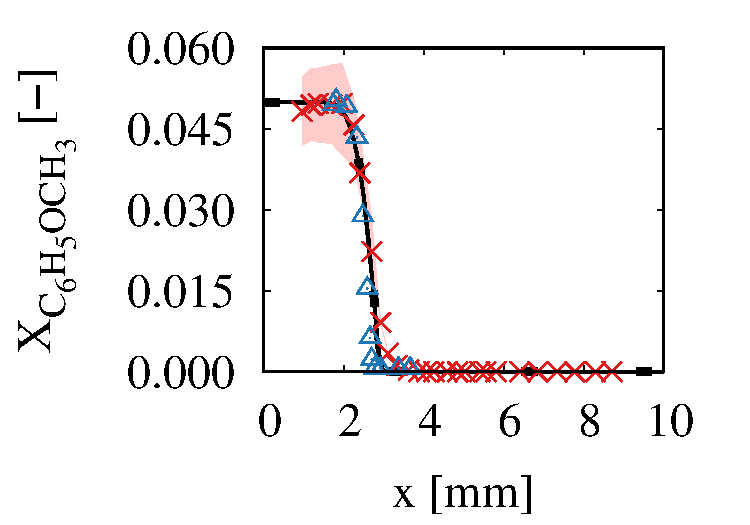
\includegraphics[width=0.32\textwidth]{\ThisPath Figures/B1b_Bio_Figure_6a.pdf}}
  \hfill
  \subfloat{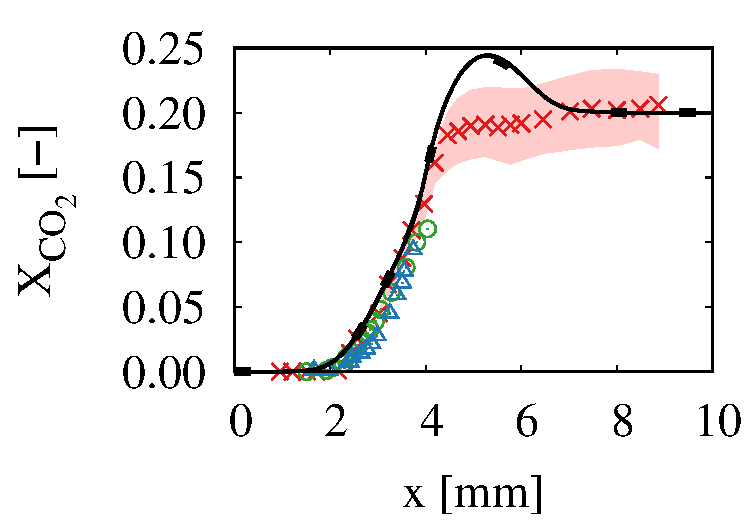
\includegraphics[width=0.32\textwidth]{\ThisPath Figures/B1b_Bio_Figure_6f.pdf}}
  \hfill
  \subfloat{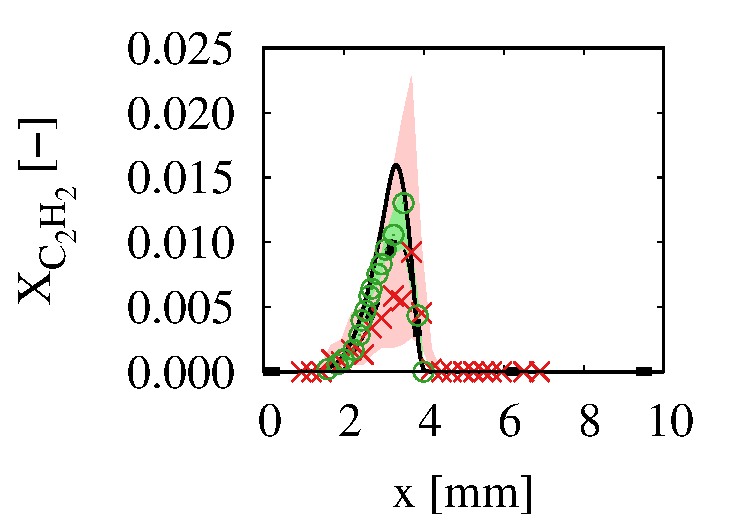
\includegraphics[width=0.32\textwidth]{\ThisPath Figures/B1b_Bio_Figure_8b.pdf}}
  \caption{Comparison of experimentally measured mole fractions in the \ce{CO2}-O-Flame for anisole oxidation from Chen et al.~\cite{Chen2022} (Time-of-Flight Molecular Beam Mass Spectrometer (ToF-MBMS): red crosses; Gas Chromatograph Mass Spectrometer (GC-MS) with a Rt-Q-Bond column: green circles; GC-MS with a DB-Petro column: blue triangles) with model predictions of the Skeletal-ITV-Bio (solid lines), the Merged-ITV-Anisole (dotted lines). Shaded areas with different colours indicate the measurement uncertainty of the respective techniques. x refers to the distance from the fuel inlet at 0 mm to the oxidiser inlet at 10 mm.}
  \label{fig:B1bAnisoleOxidationBioMechanismOXY}
\end{figure}
\\
Model validation for the secondary pyrolysis of volatile cellulose species at different temperature levels is shown in Fig.~\ref{fig:B1bCellulosePyrolysisBioMechanism} in comparison to the Merged-ITV-Cellulose and the CRECK-Bio model~\cite{Debiagi2016}. Model predictions between the Skeletal-ITV-Bio and the Merged-ITV-Cellulose show only minor discrepancies. The discrepancies shown for benzene \ce{A1} between the Merged-ITV-Cellulose and the CRECK-Bio model~\cite{Debiagi2016} at higher temperatures result from the different base chemistries.
\\
The lignin combustion part of the Skeletal-ITV-Bio model is validated with the anisole oxidation in the \ce{CO2}-\ce{O2} counterflow flame from Chen et al.~\cite{Chen2022}. Analogously to what was shown for the Skeletal-ITV-Coal model (Figure~\ref{fig:B1bAnisoleOxidationCoalMechanismCO2O}), Figure~\ref{fig:B1bAnisoleOxidationBioMechanismOXY} compares the experimental measurements with the model predictions of the Skeletal-ITV-Bio model, the Merged-ITV-Anisole, and the LLNL-Anisole model~\cite{Wagnon2018}. Anisole and \ce{CO2} mole fractions are well predicted with the Skeletal-ITV-Bio model, while the \ce{C2H2} formation is slightly over-predicted in comparison to the Merged-ITV-Anisole as shown in Fig.~\ref{fig:B1bAnisoleOxidationBioMechanismOXY}.


\subsection{\ce{NOx} chemical kinetic sub-model}

\ce{NO_x} formation is validated for the Skeletal-ITV-\ce{NO_x} model for the volatile species released from the solid particle sub-model described in chapter 8 in a predefined range of validity against experimental data~\cite{Wu2022}.
\begin{figure}[t]
  \centering
  \subfloat{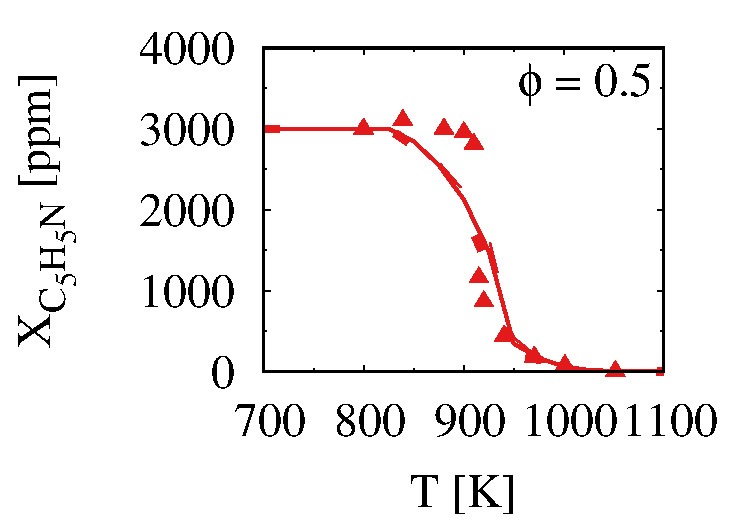
\includegraphics[width=0.32\textwidth]{\ThisPath Figures/B1b_NOx_Wu_Lean_C5H5N.pdf}}
  \hfill
  \subfloat{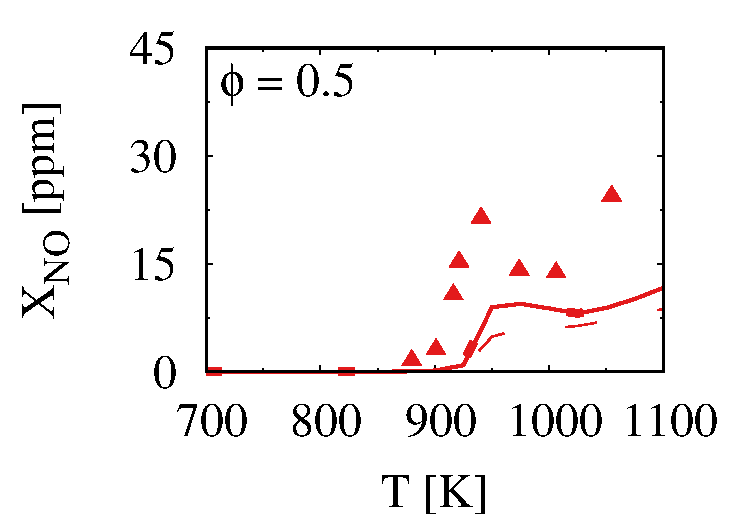
\includegraphics[width=0.32\textwidth]{\ThisPath Figures/B1b_NOx_Wu_Lean_NO.pdf}}
  \hfill
  \subfloat{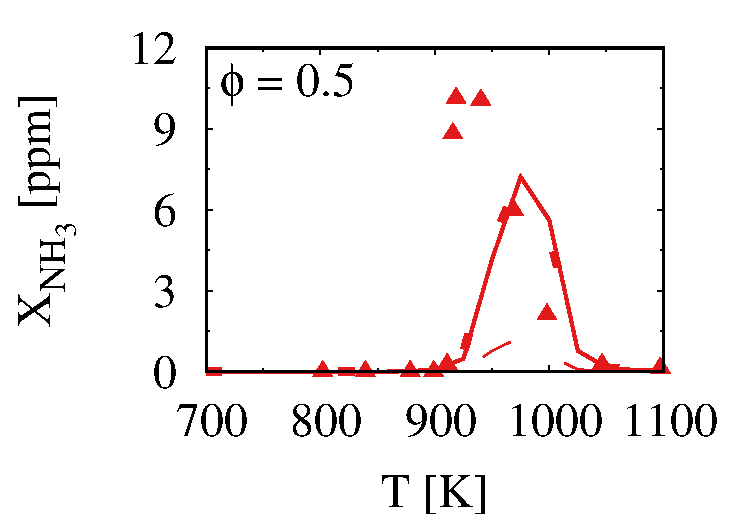
\includegraphics[width=0.32\textwidth]{\ThisPath Figures/B1b_NOx_Wu_Lean_NH3.pdf}}
  \caption{Comparison of experimental data from Wu et al.~\cite{Wu2022} in a jet-stirred reactor (symbols) with model predictions of the Skeletal ITV-\ce{NO_x} (solid lines), the Complete-ITV-\ce{NO_x} (dotted lines), and the CRECK-\ce{NO_x} model~\cite{Shamooni2021} (dashed lines).}
  \label{fig:B1bNOxWuValidation}
\end{figure}
\\
Figure~\ref{fig:B1bNOxWuValidation} compares the model predictions of the Skeletal-ITV-\ce{NO_x} with the model predictions of the Complete-ITV-\ce{NO_x} and the CRECK-\ce{NO_x} model~\cite{Shamooni2021} and with experimental measurements for fuel-lean conditions from Wu et al.~\cite{Wu2022}. The integrated \ce{C5H5N}-chemistry shows no discrepancies. In contrast, the \ce{NO} and \ce{NH3} model predictions from the ITV-based models are closer to the experimental measurements under these conditions than the CRECK-\ce{NO_x} model~\cite{Shamooni2021} predictions. Model predictions of the Skeletal-ITV-\ce{NO_x} and the Compact-ITV-\ce{NO_x} model show no discrepancies, indicating that the neglected pathways in the reduction step have only a minor error in the prediction accuracy of the target species.

\input{\ThisPath ../A1/BioCPDGasphase.tex}

\newpage
\section{Conclusions}

In this chapter, the importance of chemical kinetics models to describe the gas-phase of combustion phenomena has been addressed. In particular, developing and validating chemical kinetic models to balance the accuracy with the computational costs is a crucial aspect. To achieve this, skeletal chemical kinetic models, derived from detailed ones, are necessary. 
\\
First, a skeletal kinetic model for coal combustion was established~\cite{Cai2019, Cai2020} and validated for the ignition delay time, the laminar burning velocity, and the extinction strain rate of \ce{CH4} under air and oxy-fuel conditions. Then, new skeletal kinetic models for coal and biomass were developed by adding new species, fundamental during the volatilisation phase. Some examples of volatiles are anisole, one of the dominant volatile species released during lignin combustion, levoglucosan, dominant in cellulose combustion, and propionaldehyde, preeminent, together with anisole, at particle temperature where biomass ignites. The new coal skeletal model has been validated by considering the oxidation of anisole at atmospheric pressure over a broad range of temperatures. For the biomass model, a validation of the ignition delay time and the levoglucosan and anisole chemistry has been carried out. Furthermore, a chemical kinetic gas-phase model for \ce{NO_x} formation was built. It was crafted from a reduced version of the Glarborg model~\cite{Glarborg2018} to which the ammonia chemistry from the KAUST model and the tar-N chemistry from the CRECK-\ce{NOx} model~\cite{Shamooni2021} have been added. This newly developed model has been validated for the integrated \ce{C5H5N}-chemistry, \ce{NO} and \ce{NH3}.
\\
Finally, the role of secondary gas-phase reactions was investigated by comparing the experimental results from a fluidised bed reactor to different models (CRECK-S-B and Bio-CPD). It turned out that the predicted tar fraction was much higher than the experimentally observed one. In order to match the experimental results, some kinetic parameters had to be updated~\cite{Pielsticker2024}. Furthermore, more differences were found in the pyrolysis models when considering the division of the tar fraction by the molecular weight. This could be improved by implementing an additional fragment decomposition mechanism inside the particle.


%%%% DON'T CHANGE ANYTHING FROM HERE UNTIL NEXT MARKER!
\Acknowledgement

%\ThisPath 
\renewcommand{\bibname}{References}
\printbibliography[heading=subbibliography]

\end{refsection}
%%%% DONT CHANGE ANYTHING UNTIL HERE!
